\documentclass{extbook}[14pt]
\usepackage{multicol, enumerate, enumitem, hyperref, color, soul, setspace, parskip, fancyhdr, amssymb, amsthm, amsmath, bbm, latexsym, units, mathtools}
\everymath{\displaystyle}
\usepackage[headsep=0.5cm,headheight=0cm, left=1 in,right= 1 in,top= 1 in,bottom= 1 in]{geometry}
\usepackage{dashrule}  % Package to use the command below to create lines between items
\newcommand{\litem}[1]{\item #1

\rule{\textwidth}{0.4pt}}
\pagestyle{fancy}
\lhead{}
\chead{Answer Key for Progress Quiz 4 Version C}
\rhead{}
\lfoot{4378-7085}
\cfoot{}
\rfoot{Fall 2020}
\begin{document}
\textbf{This key should allow you to understand why you choose the option you did (beyond just getting a question right or wrong). \href{https://xronos.clas.ufl.edu/mac1105spring2020/courseDescriptionAndMisc/Exams/LearningFromResults}{More instructions on how to use this key can be found here}.}

\textbf{If you have a suggestion to make the keys better, \href{https://forms.gle/CZkbZmPbC9XALEE88}{please fill out the short survey here}.}

\textit{Note: This key is auto-generated and may contain issues and/or errors. The keys are reviewed after each exam to ensure grading is done accurately. If there are issues (like duplicate options), they are noted in the offline gradebook. The keys are a work-in-progress to give students as many resources to improve as possible.}

\rule{\textwidth}{0.4pt}

\begin{enumerate}\litem{
Determine the domain of the function below.
\[ f(x) = \frac{6}{16x^{2} +32 x + 15} \]
The solution is \( \text{All Real numbers except } x = -1.250 \text{ and } x = -0.750. \), which is option C.\begin{enumerate}[label=\Alph*.]
\item \( \text{All Real numbers except } x = a \text{ and } x = b, \text{ where } a \in [-20.11, -19.61] \text{ and } b \in [-12.18, -11.99] \)

All Real numbers except $x = -20.000$ and $x = -12.000$, which corresponds to not factoring the denominator correctly.
\item \( \text{All Real numbers.} \)

This corresponds to thinking the denominator has complex roots or that rational functions have a domain of all Real numbers.
\item \( \text{All Real numbers except } x = a \text{ and } x = b, \text{ where } a \in [-1.45, -0.86] \text{ and } b \in [-0.92, -0.03] \)

All Real numbers except $x = -1.250$ and $x = -0.750$, which is the correct option.
\item \( \text{All Real numbers except } x = a, \text{ where } a \in [-20.11, -19.61] \)

All Real numbers except $x = -20.000$, which corresponds to removing a distractor value from the denominator.
\item \( \text{All Real numbers except } x = a, \text{ where } a \in [-1.45, -0.86] \)

All Real numbers except $x = -1.250$, which corresponds to removing only 1 value from the denominator.
\end{enumerate}

\textbf{General Comment:} Recall that dividing by zero is not a real number. Therefore the domain is all real numbers \textbf{except} those that make the denominator 0.
}
\litem{
Solve the rational equation below. Then, choose the interval(s) that the solution(s) belongs to.
\[ \frac{6}{-2x + 5} + -8 = \frac{-8}{-10x + 25} \]
The solution is \( x = 2.025 \), which is option A.\begin{enumerate}[label=\Alph*.]
\item \( x \in [2.02,4.03] \)

* $x = 2.025$, which is the correct option.
\item \( x \in [-3.9,-2.5] \)

$x = -2.975$, which corresponds to not distributing the factor $-2x + 5$ correctly when trying to eliminate the fraction.
\item \( x_1 \in [0.6, 1.7] \text{ and } x_2 \in [2.02,5.03] \)

$x = 1.625 \text{ and } x = 2.025$, which corresponds to getting the correct solution and believing there should be a second solution to the equation.
\item \( x_1 \in [-3.9, -2.5] \text{ and } x_2 \in [2.02,5.03] \)

$x = -2.975 \text{ and } x = 2.025$, which corresponds to getting the correct solution and believing there should be a second solution to the equation.
\item \( \text{All solutions lead to invalid or complex values in the equation.} \)

This corresponds to thinking $x = 2.025$ leads to dividing by zero in the original equation, which it does not.
\end{enumerate}

\textbf{General Comment:} Distractors are different based on the number of solutions. Remember that after solving, we need to make sure our solution does not make the original equation divide by zero!
}
\litem{
Solve the rational equation below. Then, choose the interval(s) that the solution(s) belongs to.
\[ \frac{7}{-2x + 2} + 4 = \frac{6}{-12x + 12} \]
The solution is \( x = 1.750 \), which is option E.\begin{enumerate}[label=\Alph*.]
\item \( \text{All solutions lead to invalid or complex values in the equation.} \)

This corresponds to thinking $x = 1.750$ leads to dividing by zero in the original equation, which it does not.
\item \( x_1 \in [-0.3, 0.1] \text{ and } x_2 \in [0.75,4.75] \)

$x = -0.250 \text{ and } x = 1.750$, which corresponds to getting the correct solution and believing there should be a second solution to the equation.
\item \( x \in [-0.3,0.1] \)

$x = -0.250$, which corresponds to not distributing the factor $-2x + 2$ correctly when trying to eliminate the fraction.
\item \( x_1 \in [0.6, 1.2] \text{ and } x_2 \in [0.75,4.75] \)

$x = 1.125 \text{ and } x = 1.750$, which corresponds to getting the correct solution and believing there should be a second solution to the equation.
\item \( x \in [0.75,2.75] \)

* $x = 1.750$, which is the correct option.
\end{enumerate}

\textbf{General Comment:} Distractors are different based on the number of solutions. Remember that after solving, we need to make sure our solution does not make the original equation divide by zero!
}
\litem{
Choose the graph of the equation below.
\[ f(x) = \frac{-1}{x + 2} - 3 \]
The solution is the graph below, which is option D.
\begin{center}
    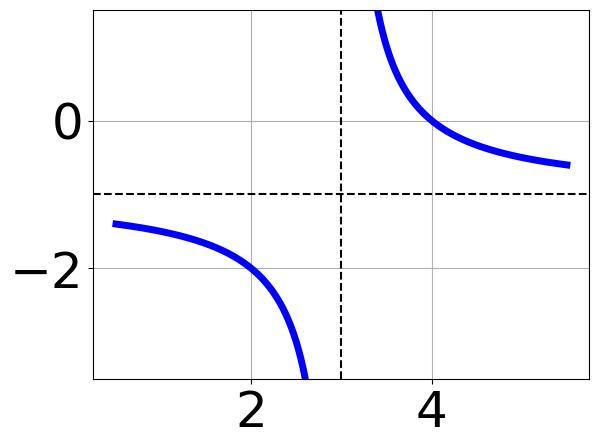
\includegraphics[width=0.3\textwidth]{../Figures/rationalEquationToGraphDC.png}
\end{center}\begin{enumerate}[label=\Alph*.]
\begin{multicols}{2}
\item 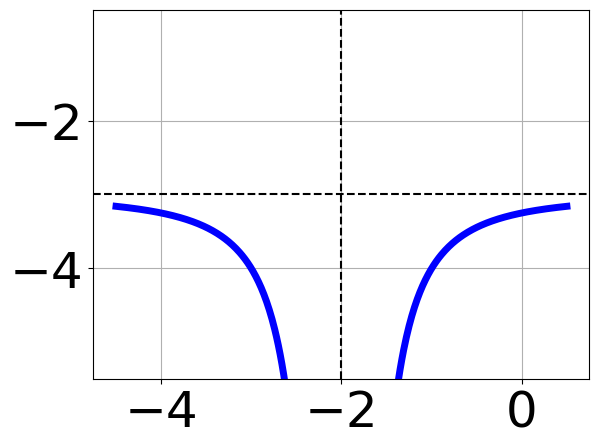
\includegraphics[width = 0.3\textwidth]{../Figures/rationalEquationToGraphAC.png}
\item 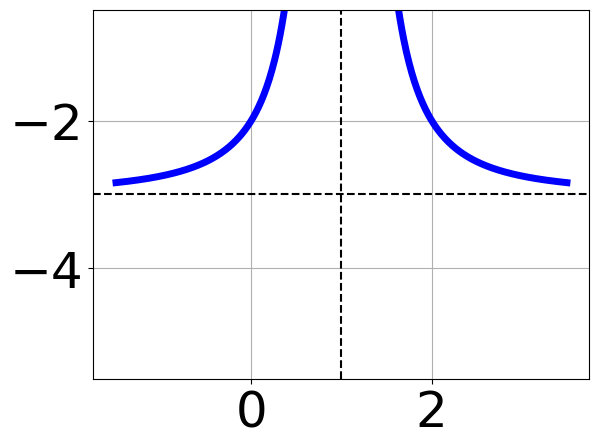
\includegraphics[width = 0.3\textwidth]{../Figures/rationalEquationToGraphBC.png}
\item 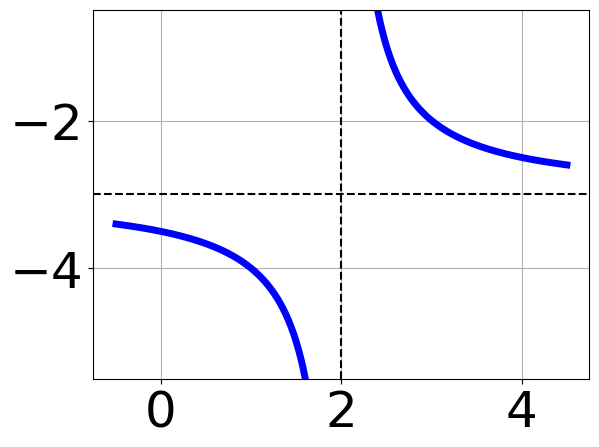
\includegraphics[width = 0.3\textwidth]{../Figures/rationalEquationToGraphCC.png}
\item 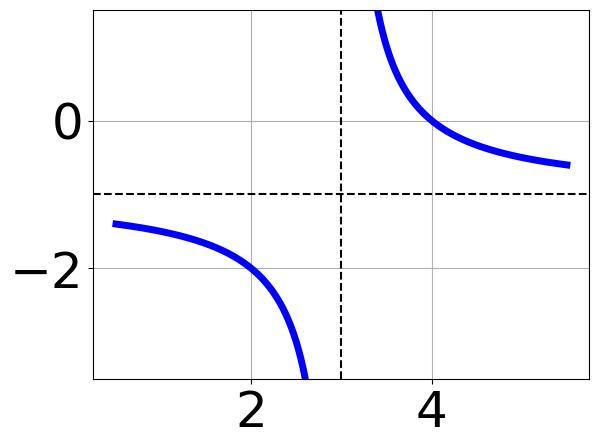
\includegraphics[width = 0.3\textwidth]{../Figures/rationalEquationToGraphDC.png}
\end{multicols}\item None of the above.\end{enumerate}
\textbf{General Comment:} Remember that the general form of a basic rational equation is $ f(x) = \frac{a}{(x-h)^n} + k$, where $a$ is the leading coefficient (and in this case, we assume is either $1$ or $-1$), $n$ is the degree (in this case, either $1$ or $2$), and $(h, k)$ is the intersection of the asymptotes.
}
\litem{
Determine the domain of the function below.
\[ f(x) = \frac{3}{20x^{2} -27 x + 9} \]
The solution is \( \text{All Real numbers except } x = 0.600 \text{ and } x = 0.750. \), which is option E.\begin{enumerate}[label=\Alph*.]
\item \( \text{All Real numbers except } x = a \text{ and } x = b, \text{ where } a \in [11.85, 12.02] \text{ and } b \in [14.48, 15.21] \)

All Real numbers except $x = 12.000$ and $x = 15.000$, which corresponds to not factoring the denominator correctly.
\item \( \text{All Real numbers.} \)

This corresponds to thinking the denominator has complex roots or that rational functions have a domain of all Real numbers.
\item \( \text{All Real numbers except } x = a, \text{ where } a \in [11.85, 12.02] \)

All Real numbers except $x = 12.000$, which corresponds to removing a distractor value from the denominator.
\item \( \text{All Real numbers except } x = a, \text{ where } a \in [0.32, 0.71] \)

All Real numbers except $x = 0.600$, which corresponds to removing only 1 value from the denominator.
\item \( \text{All Real numbers except } x = a \text{ and } x = b, \text{ where } a \in [0.32, 0.71] \text{ and } b \in [0.64, 0.85] \)

All Real numbers except $x = 0.600$ and $x = 0.750$, which is the correct option.
\end{enumerate}

\textbf{General Comment:} Recall that dividing by zero is not a real number. Therefore the domain is all real numbers \textbf{except} those that make the denominator 0.
}
\litem{
Choose the equation of the function graphed below.

\begin{center}
    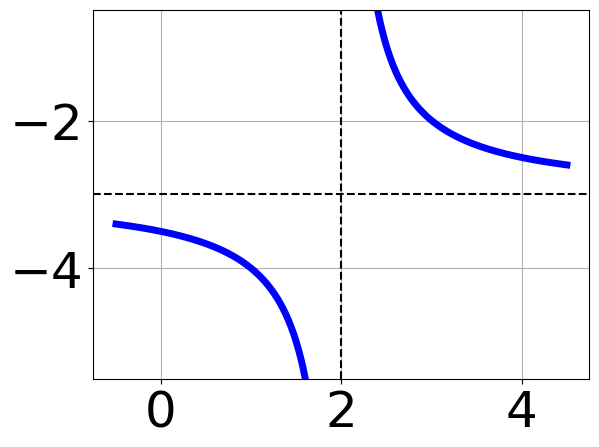
\includegraphics[width=0.5\textwidth]{../Figures/rationalGraphToEquationC.png}
\end{center}



The solution is \( \text{None of the above as it should be } f(x) = \frac{1}{(x + 2)^2} - 3 \), which is option E.\begin{enumerate}[label=\Alph*.]
\item \( f(x) = \frac{1}{x - 2} - 3 \)

Corresponds to thinking the graph was a shifted version of $\frac{1}{x}$.
\item \( f(x) = \frac{-1}{x + 2} - 3 \)

Corresponds to thinking the graph was a shifted version of $\frac{1}{x}$, using the general form $f(x) = \frac{a}{(x-h)^2}+k$, and the opposite leading coefficient.
\item \( f(x) = \frac{-1}{(x + 2)^2} - 3 \)

Corresponds to using the general form $f(x) = \frac{a}{(x-h)^2}+k$ and the opposite leading coefficient.
\item \( f(x) = \frac{1}{(x - 2)^2} - 3 \)

The $x$-value of the equation does not match the graph.
\item \( \text{None of the above} \)

None of the equation options were the correct equation.
\end{enumerate}

\textbf{General Comment:} Remember that the general form of a basic rational equation is $ f(x) = \frac{a}{(x-h)^n} + k$, where $a$ is the leading coefficient (and in this case, we assume is either $1$ or $-1$), $n$ is the degree (in this case, either $1$ or $2$), and $(h, k)$ is the intersection of the asymptotes.
}
\litem{
Solve the rational equation below. Then, choose the interval(s) that the solution(s) belongs to.
\[ \frac{-6x}{6x -5} + \frac{-7x^{2}}{-42x^{2} +71 x -30} = \frac{-2}{-7x + 6} \]
The solution is \( \text{There are two solutions: } x = -0.292 \text{ and } x = 0.978 \), which is option C.\begin{enumerate}[label=\Alph*.]
\item \( x_1 \in [-0.32, -0.23] \text{ and } x_2 \in [0.77,0.91] \)


\item \( x \in [0.95,1.01] \)


\item \( x_1 \in [-0.32, -0.23] \text{ and } x_2 \in [0.9,1.05] \)

* $x = -0.292 \text{ and } x = 0.978$, which is the correct option.
\item \( \text{All solutions lead to invalid or complex values in the equation.} \)


\item \( x \in [0.77,0.96] \)


\end{enumerate}

\textbf{General Comment:} Distractors are different based on the number of solutions. Remember that after solving, we need to make sure our solution does not make the original equation divide by zero!
}
\litem{
Solve the rational equation below. Then, choose the interval(s) that the solution(s) belongs to.
\[ \frac{2x}{5x + 7} + \frac{-7x^{2}}{20x^{2} +38 x + 14} = \frac{-6}{4x + 2} \]
The solution is \( \text{There are two solutions: } x = -32.716 \text{ and } x = -1.284 \), which is option A.\begin{enumerate}[label=\Alph*.]
\item \( x_1 \in [-34.16, -32.61] \text{ and } x_2 \in [-1.33,-1.22] \)

* $x = -32.716 \text{ and } x = -1.284$, which is the correct option.
\item \( \text{All solutions lead to invalid or complex values in the equation.} \)


\item \( x \in [-2.06,-0.99] \)


\item \( x \in [-0.66,0.49] \)


\item \( x_1 \in [-34.16, -32.61] \text{ and } x_2 \in [-1.55,-1.32] \)


\end{enumerate}

\textbf{General Comment:} Distractors are different based on the number of solutions. Remember that after solving, we need to make sure our solution does not make the original equation divide by zero!
}
\litem{
Choose the equation of the function graphed below.

\begin{center}
    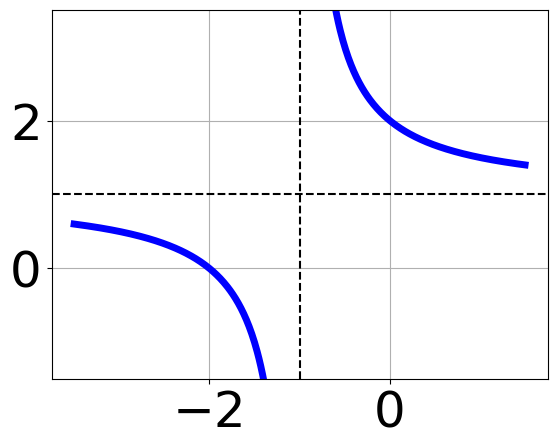
\includegraphics[width=0.5\textwidth]{../Figures/rationalGraphToEquationCopyC.png}
\end{center}



The solution is \( f(x) = \frac{-1}{x - 2} - 1 \), which is option B.\begin{enumerate}[label=\Alph*.]
\item \( f(x) = \frac{-1}{(x - 2)^2} - 1 \)

Corresponds to thinking the graph was a shifted version of $\frac{1}{x^2}$.
\item \( f(x) = \frac{-1}{x - 2} - 1 \)

This is the correct option.
\item \( f(x) = \frac{1}{x + 2} - 1 \)

Corresponds to using the general form $f(x) = \frac{a}{x+h}+k$ and the opposite leading coefficient.
\item \( f(x) = \frac{1}{(x + 2)^2} - 1 \)

Corresponds to thinking the graph was a shifted version of $\frac{1}{x^2}$, using the general form $f(x) = \frac{a}{x+h}+k$, and the opposite leading coefficient.
\item \( \text{None of the above} \)

This corresponds to believing the vertex of the graph was not correct.
\end{enumerate}

\textbf{General Comment:} Remember that the general form of a basic rational equation is $ f(x) = \frac{a}{(x-h)^n} + k$, where $a$ is the leading coefficient (and in this case, we assume is either $1$ or $-1$), $n$ is the degree (in this case, either $1$ or $2$), and $(h, k)$ is the intersection of the asymptotes.
}
\litem{
Choose the graph of the equation below.
\[ f(x) = \frac{-1}{x - 2} + 2 \]
The solution is the graph below, which is option E.
\begin{center}
    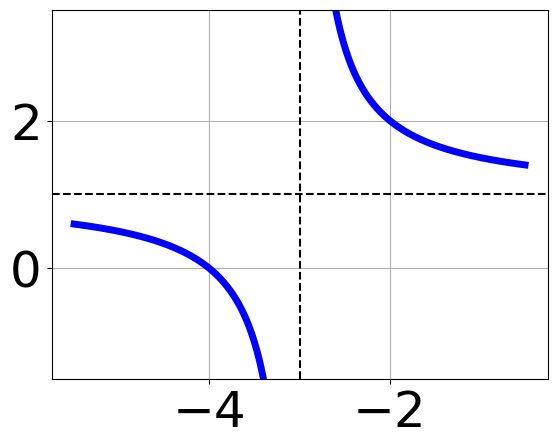
\includegraphics[width=0.3\textwidth]{../Figures/rationalEquationToGraphCopyEC.png}
\end{center}\begin{enumerate}[label=\Alph*.]
\begin{multicols}{2}
\item 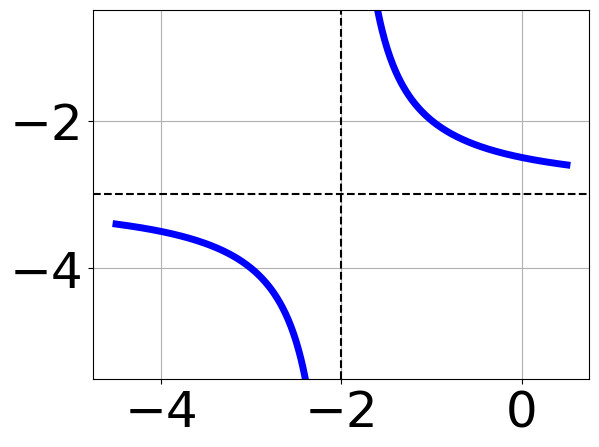
\includegraphics[width = 0.3\textwidth]{../Figures/rationalEquationToGraphCopyAC.png}
\item 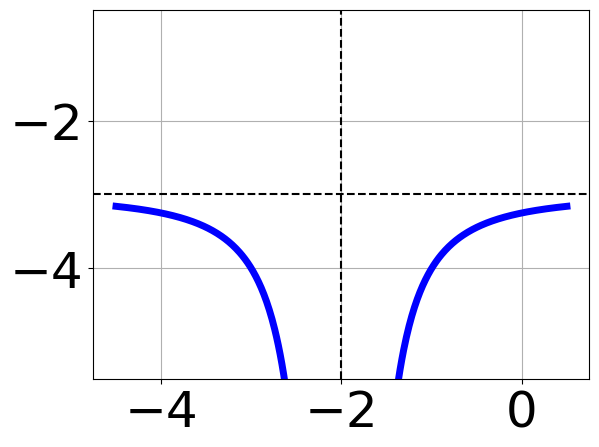
\includegraphics[width = 0.3\textwidth]{../Figures/rationalEquationToGraphCopyBC.png}
\item 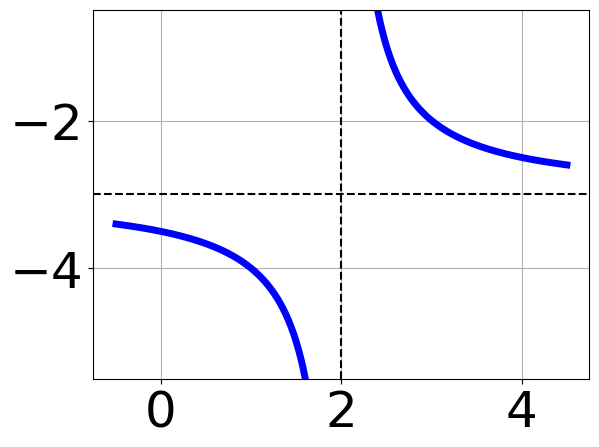
\includegraphics[width = 0.3\textwidth]{../Figures/rationalEquationToGraphCopyCC.png}
\item 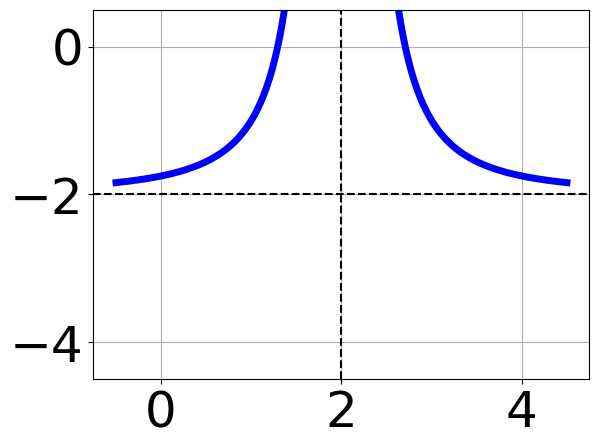
\includegraphics[width = 0.3\textwidth]{../Figures/rationalEquationToGraphCopyDC.png}
\end{multicols}\item None of the above.\end{enumerate}
\textbf{General Comment:} Remember that the general form of a basic rational equation is $ f(x) = \frac{a}{(x-h)^n} + k$, where $a$ is the leading coefficient (and in this case, we assume is either $1$ or $-1$), $n$ is the degree (in this case, either $1$ or $2$), and $(h, k)$ is the intersection of the asymptotes.
}
\end{enumerate}

\end{document}